\documentclass[12pt,twoside,book]{article}

\input{../settings}

\begin{document}

%%%%%%%%%%%%%%%%%%%%%%%%%%%%%%%%%%%%%%%%%%%%%%%%%%%%%%%%%%%%%%%%%%%%%%%%%%%%%%%
\section{Properties of the transverse mass}
\label{sec:mT}
%%%%%%%%%%%%%%%%%%%%%%%%%%%%%%%%%%%%%%%%%%%%%%%%%%%%%%%%%%%%%%%%%%%%%%%%%%%%%%%

In this appendix, we summarize the properties of the transverse mass, which is used for the analysis of the mono-lepton final state in Sec.~\ref{sec:dy}.
The transverse mass is a useful quntity when there is a unique invisible particle (which we will call $I$) such as a neutrino in the final state.
As already mentioned in Sec.~\ref{sec:WIMP}, the transverse mass $m_T$ is defined event by event using the measured value of the missing transverse momentum $\Slash{E}_{T}$ as
\begin{align}
  m_T^2 \equiv 2 p_T\,\Slash{E}_T \left( 1-\cos \phi \right),
\end{align}
where $p_T$ denotes the transverse momentum of a (visible) final state particle (which will call $P$) and $\phi$ is the difference between the azimuth angles of $p_T$ and $\Slash{E}_T$.
It is important that we can infer the invariant mass of particles $P$ and $I$ with $m_T$, if both $P$ and $I$ are (approximately) massless.

Let $p_P$ and $p_I$ be the four momenta of $P$ and $I$, respectively.
When there is only one invisible particle in the event, the transverse part of $p_I$ is roughly identified with $\Slash{E}_T$.
Hereafter, we assume the exact equality among them just for simplicity, which corresponds to neglect the detector errors, transverse momentum of initial partons, soft emissions that is invisible for detectors, and so on.
Then, we can write the components of four momenta as
\begin{align}
  p_P &= \left( E_P, p_T \cos\phi_P, p_T \sin\phi_P, p_{Pz} \right),\\
  p_I &= \left( E_I, \Slash{E}_T \cos\phi_I, \Slash{E}_T \sin\phi_I, p_{Iz} \right),
\end{align}
with $\phi \equiv \phi_P - \phi_I$.
Note that massless conditions are satisfied, namely $E_P^2 = p_T^2 + p_{Pz}^2$ and $E_I^2 = \Slash{E}_T^2 + p_{Iz}^2$.
We can derive a relation between $m_T$ and $m_{PI} \equiv \sqrt{(p_P + p_I)^2}$
\begin{align}
  m_T \leq m_{PI},
\end{align}
where the equation holds when
\begin{align}
  p_{Pz} \Slash{E}_T - p_T p_{Iz} = 0.
  \label{eq:mT_equality}
\end{align}
When the above equation roughly holds, $m_{PI} - m_T$ glows proportional to the quadratic of the left-handed side of Eq.~\eqref{eq:mT_equality}.

It is more intuitive to understand the situation in the center of mass system (CMS), focusing on the pair production process of particles $P$ and $I$.
In this case, the transverse momentum of the event is simply given by
\begin{align}
  m_T^{\mathrm{(CMS)}} = m_{PI} \sin \theta^{(\mathrm{CMS})},
  \label{eq:mT_CMS}
\end{align}
where $\theta^{(\mathrm{CMS})}$ is the angle between the momentum of $P$ and the beam line in the CMS.
Although the definition of $m_T$ is not Lorentz invariant and generally $m_T^{\mathrm{(CMS)}} \neq m_T$, the former gives a good approximation of the latter when the two-particle system is not highly boosted.
Let us simply assume $m_T = m_T^{\mathrm{(CMS)}}$ and consider the repeated production of $P$ and $I$ with fixed $m_{PI}$.
When we postulate the uniform distribution of the production cross section against $\cos \theta^{(\mathrm{CMS})}$ for simplicity, the distribution of the transverse mass $f(m_T)$ calculated according to Eq.~\eqref{eq:mT_CMS} possesses a sharp peak at $m_T = m_{PI}$, described by
\begin{align}
  f(m_T) =\frac{m_T}{m_{PI}}
  \cos^{-1} \left[ \arcsin \left( \frac{m_T}{m_{PI}} \right) \right].
\end{align}
This peak, often called as the Jacobian peak, enables us to estimate $m_{PI}$ from $m_T$.

\begin{figure}[t]
  \centering
  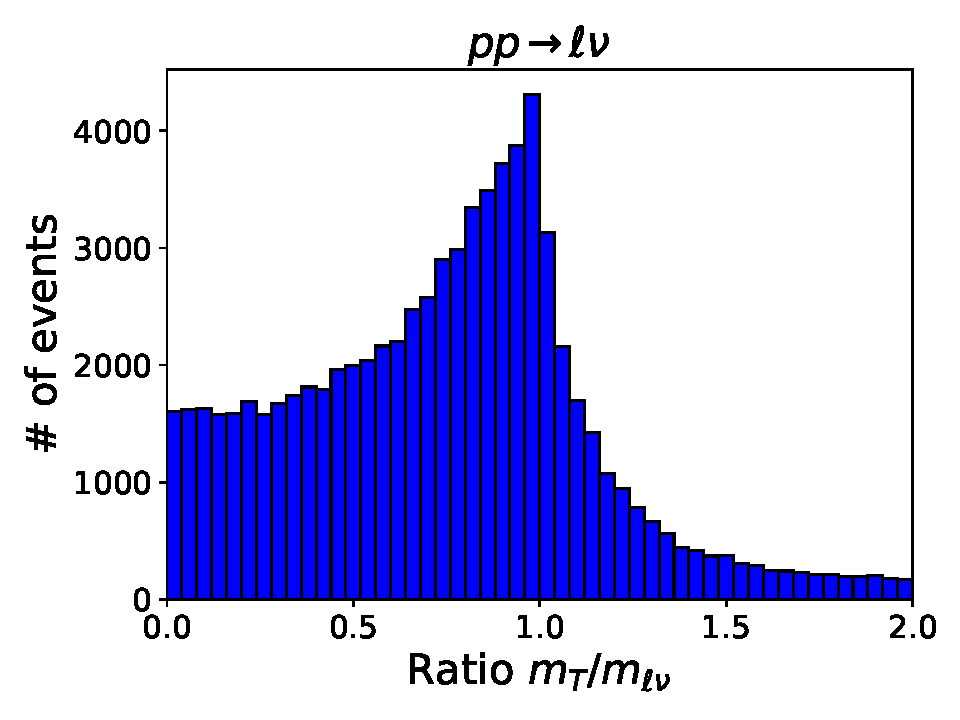
\includegraphics[width=0.5\hsize]{invariant_vs_transverse.pdf}
  \caption{
    Distribution of $m_T / m_{\ell \nu}$ for the pair production process of $P=\ell$ and $I=\nu$.
    Figure for $\sqrt{s}=100\,\mathrm{TeV}$ and $\mathcal{L}=1\,\mathrm{ab}^{-1}$.
  }
  \label{fig:invariant_vs_transverse}
\end{figure}

In Fig.~\ref{fig:invariant_vs_transverse}, we show the distribution of the ratio $m_T / m_{\ell \nu}$ for the pair production process of $P=\ell$ and $I=\nu$.
We use the setup of $\sqrt{s}=100\,\mathrm{TeV}$ and $\mathcal{L}=1\,\mathrm{ab}^{-1}$.
To evaluate the missing transverse momentum $\Slash{E}_T$ for each event, we have performed the detector simulation using \texttt{Delphes} similar to the analysis in Sec.~\ref{sec:dy}.
We can clearly see the peak at $m_T / m_{\ell \nu} = 1$, though it is somewhat smeared compared with that expected in the CMS due to the effect of the Lorentz boost and the non-trivial angular dependence of the production cross section.
Besides, the small tail of the distribution for $m_T > m_{\ell \nu}$ can be understood by the effects we have neglected so far, such as the detector errors.

\end{document}
